% !TEX root = tesis.tex

\chapter{Desarrollo de nueva electrónica para el SciCRT}
\chaptermark{Nueva electrónica}
\label{chap:tres}

Las necesidades del SciCRT operando en Sierra Negra no se acoplan directamente a los objetivos específicos de los experimentos K2K y SciBooNE, una de nuestras metas dentro de la colaboración ha sido el desarrollo de electrónica de alta velocidad de transferencia, bajo costo y consumo de potencia. Sumado a esto, hemos decido seguir principios similares a los del desarrollo de software libre para evitar el \emph{vendor lock-in}. No obstante, encontrar una solución que cumpla de forma simultánea todos estos requerimientos resulta muy complejo. En este capítulo abordaré detalladamente el desarrollo del sistema de adquisición de datos, dando particular énfasis a su motivación científica. En este sentido el primer punto a tratar será la velocidad de transferencia.

En \num{2015} desarrollamos nueva electrónica BE utilizando \emph{SiTCP} (procesador embebido programable desarrollado para experimentos de física de altas energías \cite{uchida08}) y la instalamos en uno de los SB que componen las capas de neutrones del telescopio \cite{ysasai17}. Gracias al uso de esta tecnología logramos alcanzar una tasa de transferencia de datos \num{10} veces mayor a la que teníamos con el bus VME.

A continuación presento un estudio mediante simulación MC para evaluar el desempeño del SciCRT utilizando la electrónica de alta velocidad. Este análisis tiene también por objetivo mostrar la motivación detrás del requerimiento en la velocidad de transferencia. Hago notar que estudios similares se encuentran en: \cite{ynagai14,ysasai17}. El resultado original contenido en esta tesis lo presenté en la Conferencia internacional de Rayos Cósmicos en \emph{Busan}, Corea del Sur \cite{manzorena171}.

\section{Desempeño del SciCRT ante un evento de neutrones solares}

Evaluaremos la respuesta del SciCRT a un evento de neutrones solares mediante simulación MC, comparando el resultado con los datos obtenidos por el TNS instalado en Sierra Negra durante la ráfaga del \num{7} de Septiembre de \num{2005} \cite{sako06}. Este evento fue detectado por el TNS con una significacia de $17\sigma$ en el canal de partículas neutras con energías mayores a $>\SI{30}{\mega\electronvolt}$. El pico de la emisión de rayos \emph{X} duros (satélite Integral) fue a las 17:36:40 UT. La figura

Si asumimos el flujo de neutrones solares para este evento, podemos estimar la significancia de las señales detectadas por el SciCRT en un evento similar. Para nuestra estimación consideraremos como parámetros de entrada \cite{ynagai14}: un espectro de energía de los neutrones en el Sol de acuerdo a una ley de potencias
$\num{6.1e27}\left(E/\si{\mega\electronvolt}\right)^{-3.8}\si{\per\mega\electronvolt\per\steradian}$, neutrones emitidos de manera impulsiva en el Sol y un ángulo cenital de \ang{17.5}. La propagación de los neutrones solares en la atmósfera terrestre se simula usando el modelo de Shibata.

\begin{figure}
\centering
  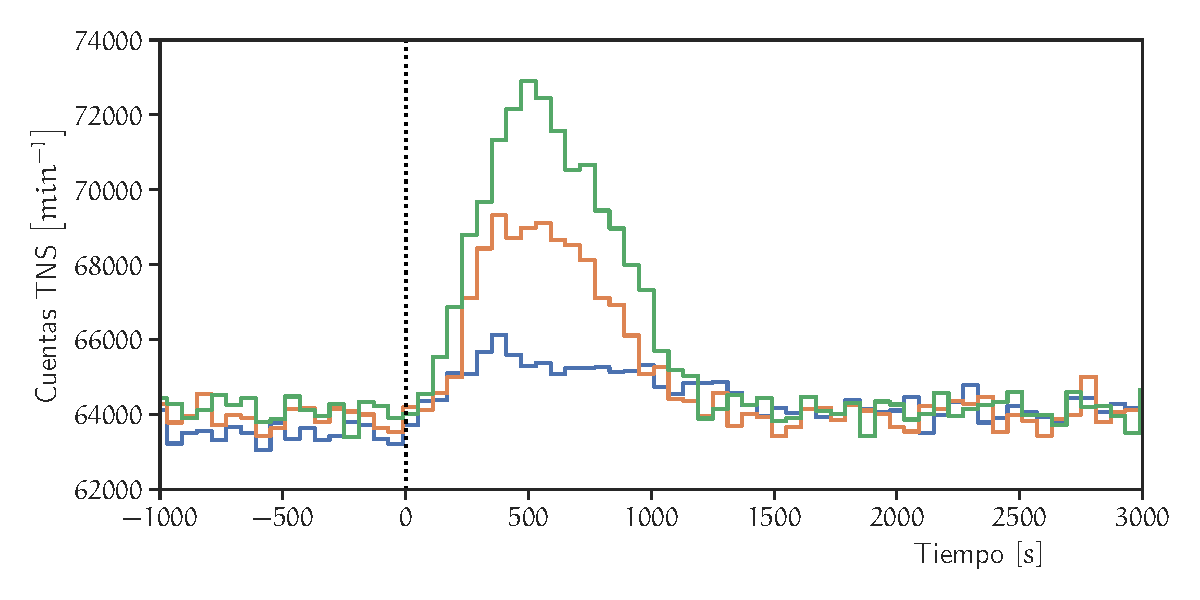
\includegraphics[width=\textwidth]{scicrt-sim.pdf}
  \caption{Simulación de los perfiles temporales del SciCRT asumiendo un flujo de neutrones solares similar al del evento del \num{7} de Septiembre de \num{2005}. La curva azul muestra los datos obtenidos por el TNS, la línea naranja es el perfil temporal del SciCRT usando la electrónica original. La línea roja muestra el caso cuando instalamos la electrónica de alta velocidad. Los datos están normalizados al nivel de fondo del TNS.}
  \label{fig:solar-sim}
\end{figure}

Los resultados de nuestro cálculo se muestran en la figura \ref{fig:solar-sim}. Es importante aclarar que para esta estimación tomamos en cuenta dos situaciones; una con la electrónica original y otra con la electrónica de alta velocidad, ambas instaladas en $4/8$ del detector. La línea punteada en \SI{0}{\second} indica el instante en que la intensidad de rayos \emph{X} duros alcanzó el máximo. En la figura la linea azul representa los datos del TNS de partículas neutras con $E_{k}>\SI{30}{\mega\electronvolt}$. El perfil temporal de las cuentas del SciCRT con la electrónica original (línea naranja) muestra una significacia de $39\sigma$, lo que se traduce en una sensibilidad \num{2.3} veces mayor a la del TNS durante el mismo evento. Sin embargo, al tomar en cuenta el caso de la nuevo DAQ (línea verde), el incremento es de $59\sigma$, es decir, \num{3.5} veces mayor sensibilidad.

Con respecto a los datos de energía depositada (considerando el uso de electrónica de alta velocidad) el incremento también notable puesto que se tiene una sensibilidad \num{3} veces mayor, con la ventaja extra de que podemos estimar el espectro de los neutrones con una excelente resolución \cite{ysasai17}.

A pesar de este resultado positivo, la sensibilidad del detector es directamente función del volumen activo del telescopio. Para justificar este punto, la figura \ref{fig:eficiencia-electronica} muestra la eficiencia de detección de neutrones en función del número de SB instalados y la energía incidente. Las línea azul representa el caso para un SB, la línea naranja dos SB y la verde cuatro. De la figura es posible concluir que la eficiencia de detección de neutrones incrementa principalmente en la zona de bajas energías ($<$\SI{100}{\mega\electronvolt}). Este resultado concuerda con lo expuesto en \cite{nagaiphd}, el cual reporta una eficiencia del \SI{30}{\percent} para neutrones de \SI{50}{\mega\electronvolt}. En el caso de los neutrones de mayor energía, aunque la eficiencia de detección no tiene un incremento tan significativo con el número de SBs instalados, las capacidades para estudiar el espectro de energía y la distribución angular si son enormemente mejoradas con la instalación de nueva electrónica.

Adicionalmente, dada la operación del telescopio en alta montaña, la operación sostenible a largo plazo requiere de la producción de electrónica de bajo costo y potencia de consumo, ya que las condiciones ambientales reducen la vida útil de los componentes, además de dificultar la disipación de calor. Tomando en cuenta todo lo anterior y considerando que solo $3/8$ de la electrónica total necesaria para la instalación está disponible en estos momentos, el desarrollo de nuevas unidades de \emph{front end} se vuelve una prioridad de nuestro experimento.

\begin{figure}
        \centering
        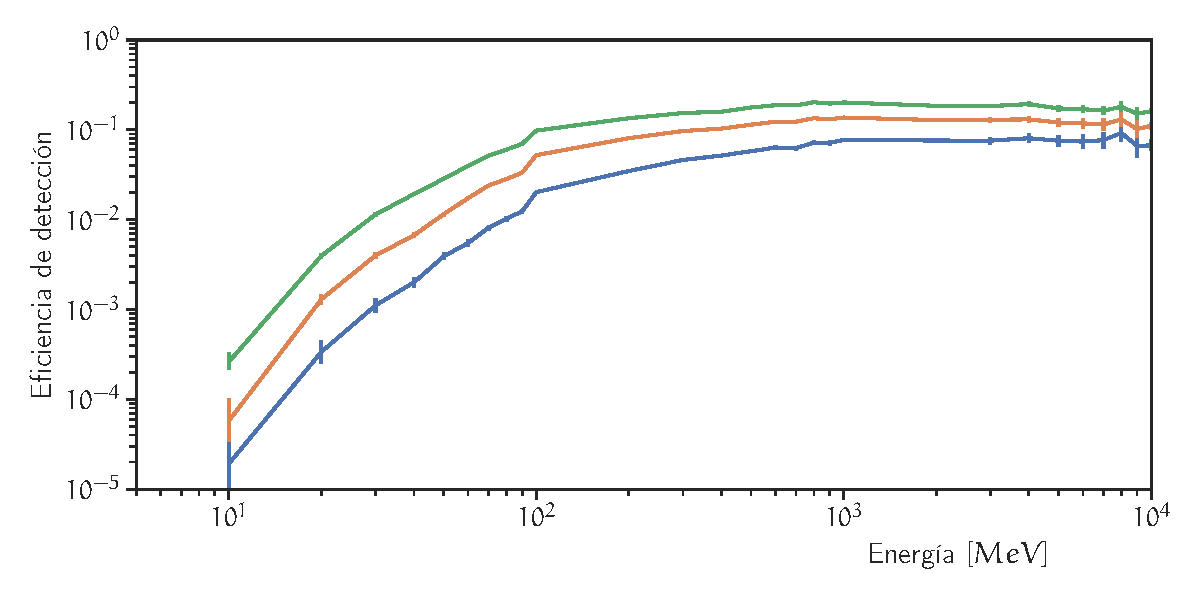
\includegraphics[width=\textwidth]{electronics-deff.pdf}
        \caption{Eficiencia de detección de neutrones en función de SB instalados. La gráfica azul representa la eficiencia con un SB, la gráfica naranja es con dos SB y la verde con cuatro SB.}
        \label{fig:eficiencia-electronica}
\end{figure}

\section{La técnica de \emph{Time over threshold}}

Como mencioné en el capitulo \ref{chap:dos}, cuando una partícula energética entra en el volumen activo de un detector, ésta pierde su energía interaccionando con el medio. Considerando una partícula con carga eléctrica, la energía depositada se puede estimar midiendo las pérdidas por ionización; el número de iones generados al atravesar el detector. En el caso de un material centellador la medida de la pérdida por ionización es el número de fotones.

De esta forma, el cálculo de la carga depositada $Q$ en el detector se puede realizar integrando la señal de corriente:

\begin{equation}
\label{equ:charge}
Q=\int_{0}^{T_{max}} i_{pmt}\left(t\right)\mathrm{d}t
\end{equation}

de donde $T_{max}$ es el tiempo de corte, el cual se debe escoger la más grande posible para garantizar que la integración incluya la mayor cantidad de fotoelectrones\footnote{Idealmente este tiempo debe ser infinito, sin embargo esto lleva a la saturación de la electrónica.}. Luego entonces, una método sencillo para procesar este tipo de información consiste en integrar los pulsos para posteriormente digitalizarlos. Esto constituye la base de las técnicas convencionales de procesamiento de pulsos utilizadas ampliamente en electrónica nuclear.

Con la llegada de sistemas de detección de radiación de gran escala (sistemas de miles de canales o más), los métodos basados en digitalización de pulsos se implementan en circuitos de aplicación específica (ASIC); lo cual permite una excelente resolución de energía, bajo consumo de potencia y tamaño reducido; a expensas de altos costos de producción y desarrollo.

Por esta razón el desarrollo de la instrumentación del SciCRT requiere de un método de estimación de energía que se adapte a las necesidades de nuestro experimento.

Una alternativa es el uso de la técnica de Time over threshold (TOT), la cual permite una arquitectura simplificada a cambio de un pérdida en la linealidad y compresión en el rango dinámico \cite{fujiwara10}. En este método una señal digital variante en el tiempo $T_{OT}$ codifica la información de la amplitud del pulso, a partir del tiempo dura el pulso analógico por encima de un umbral predefinido. Posteriormente se necesita convertir la información temporal a valores digitales usando un \emph{time digital converter} (TDC).

Para aplicar este método el primer paso será encontrar una relación entre $Q$ y $TOT$, lo cual se puede hacer resolviendo un sistema de ecuaciones no lineales. Si consideramos $s\left(t\right)$ la señal con la información de la carga y $v\left(t\right)$ la función que describe al umbral, el sistema de ecuaciones se puede escribir como:

\begin{equation}
\label{equ:tot-equ}
\begin{aligned}
\left. s\left(t\right)\right|_{t=ti} &= \left. v\left(t\right)\right|_{t=ti}\\
\left. s\left(t\right)\right|_{t=tf} &= \left. v\left(t\right)\right|_{t=tf}
\end{aligned}
\end{equation}

donde $t_{i}$ y $t_{f}$ representan los puntos en que la señal rebasa el umbral. Es importante notar que $T_{OT}=t_{f}-t_{i}$. Resolviendo este sistema para el caso particular de un pulso de centelleo del tipo exponencial obtenemos:

\begin{equation}
\begin{aligned}
ToT &= -\ln\left(\dfrac{V_{th}}{s_{0}}\right)^{\tau}\\
 &= \tau_{d} \ln\left(s_{0}\right)-K
\end{aligned}
\end{equation}

de donde $s_{0}$ representa la distribución de amplitudes del pulso (energía depositada) y $\tau$ la constante del centellador. Con este modelo simplificado podemos observar que la relación entre la carga y el TOT no es lineal. Para verificar este comportamiento realizaremos una simulación de primeros principios tomando las características similares a las de las señales del SciCRT. Primero consideramos que $s_{0}$ es una variable aleatoria distribuida normalmente $X\ \sim\ \mathcal{N}\left(\mu,\,\sigma^2\right)$, con media $\mu$ y desviación estándar $\sigma$.

El resultado de la simulación se presenta en la figura \ref{fig:tot-model}. Los paneles superior en inferior izquierdo los pulsos simulados y la distribución de amplitudes, respectivamente. Por otro lado, el panel superior derecho en la figura muestra la relación que existe entre $Q$ y $T_{OT}$ para las señales descritas. El panel inferior derecho muestra la distribución de los valores de $T_{OT}$. Idealmente la distribución debe ser la misma que en el panel izquierdo, sin embargo, debido a la relación no lineal entre $Q$ y $T_{OT}$, observamos una distorsión en el área de baja energía, lo cual limita el rango dinámico del método.

Esta limitante del método nos obliga a ser cuidadosos en la elección de parámetros de diseño de nuestro sistema, ya que sin un análisis detallado se corre el riesgo perder resolución en energía. Como expondré más adelante, esto me motivo a realizar un estudio mediante simulación buscando optimizar los parámetros de diseño.

\begin{figure}
        \centering
        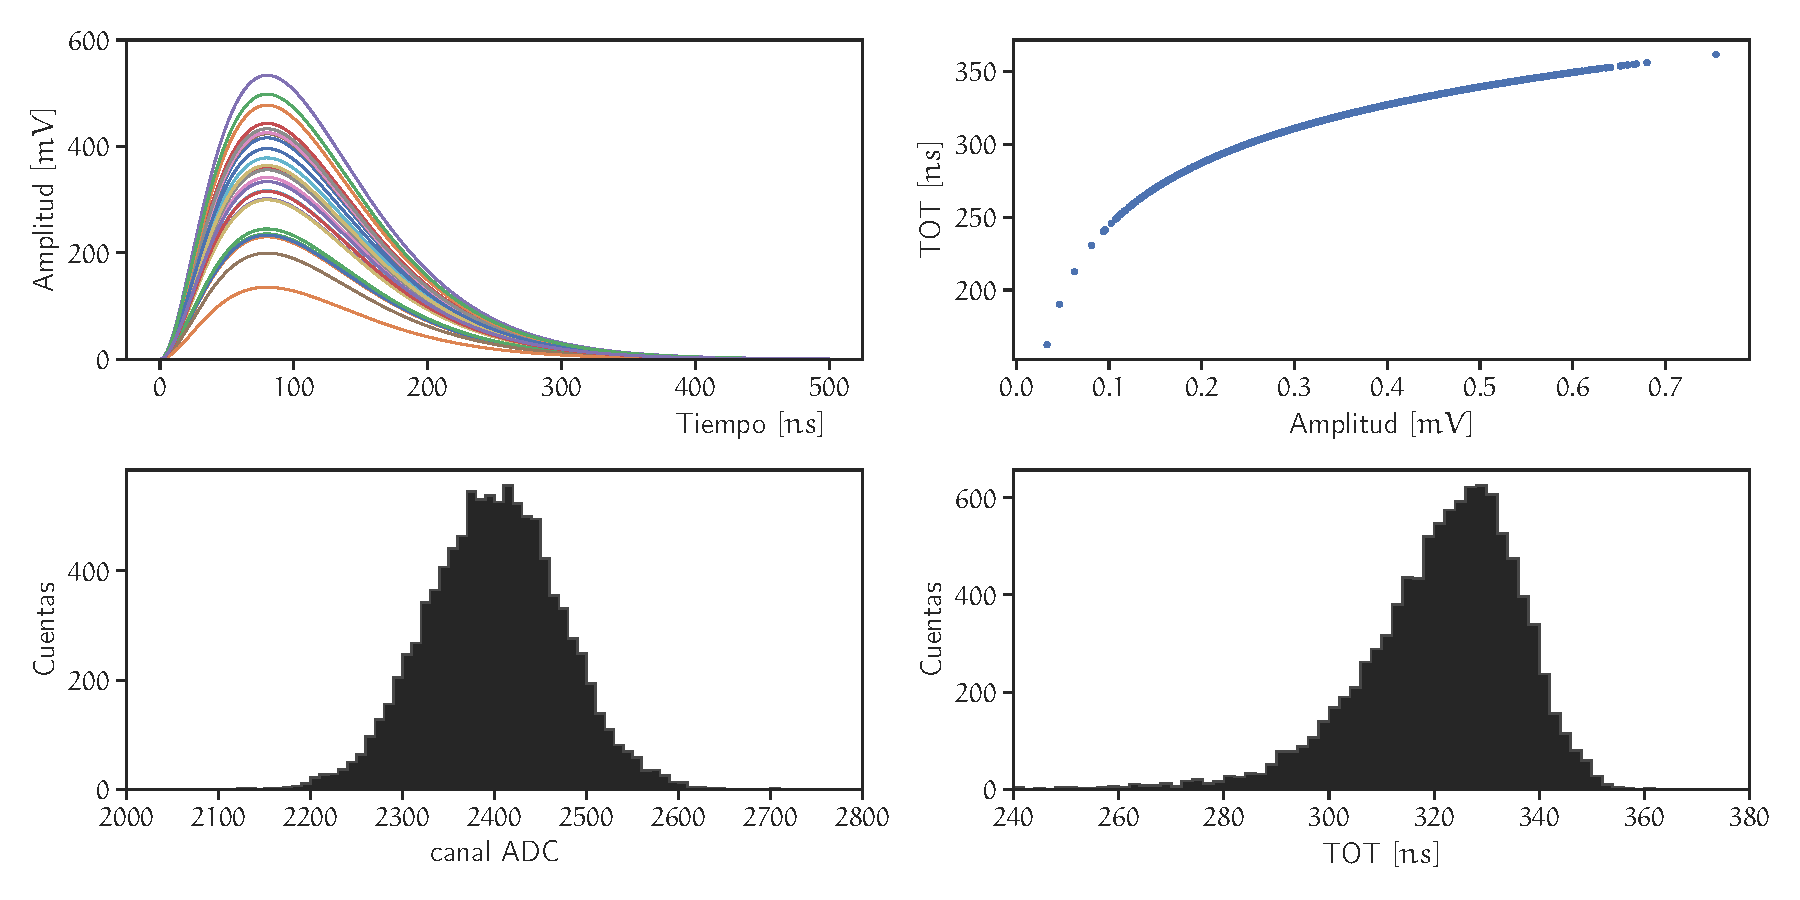
\includegraphics[width=\textwidth]{TOT-model.pdf}
        \caption{Modelo de primeros principios de conversión Carga-TOT.}
        \label{fig:tot-model}
\end{figure}

Aunado a este problema es importante establecer que la señal a la salida del detector no es útil para extraer la información de la carga depositada del evento de radiación ya que es de corta duración. Debido a esto, el primer paso antes de poder procesar la señal de radiación, es acondicionar la señal para que tenga una mayor duración y una amplitud máxima definida. El efecto de incrementar la duración de la señal, mejora la razón señal a ruido, mientras que la amplitud definida permite la lectura correcta de la información de la carga. Esto conlleva a que el proceso de optimización requiera el estudio de los diversos elementos que comprenden el sistema.

El diagrama esquemático del sistema TOT propuesto se muestra en la figura \ref{fig:nfeb-prot}. El uso de un dispositivo programable como el FPGA (field programmable gate array) permite la integración de la mayoría de las funciones requeridas por el sistema de procesamiento de pulsos, incluido SiTCP que nos permite hacer la transferencia de datos rápida. La principal ventaja de esta integración es que permite reducir el costo de desarrollo y producción.

La parte analógica del sistema está compuesta por un ciruito preamplificador y un formador.  El pramplificador tiene como función convertir la señal de corriente del fotomultiplicador en una señal de voltaje, llevando a cabo en el proceso la integración de la señal de corriente. El formador es filtro pasa banda, en el cual además de amplificar la señal de la etapa anterior, también define las características temporales (tiempos de subida, bajada y duración) de la señal del detector. Considerando que la mayor parte del sistema es digital, y que ésta se puede implementar en un sólo dispositivo: el tamaño de la tarjeta queda principalmente definido por el número de componentes utilizados para construir la sección de procesamiento analógico.

Con el fin de alcanzar una buena resolución temporal y un bajo uso de los recursos del circuito programable, para el diseño del TDC escogí la técnica de sobremuestreo que se describe en la siguiente sección.

\begin{figure}
        \centering
        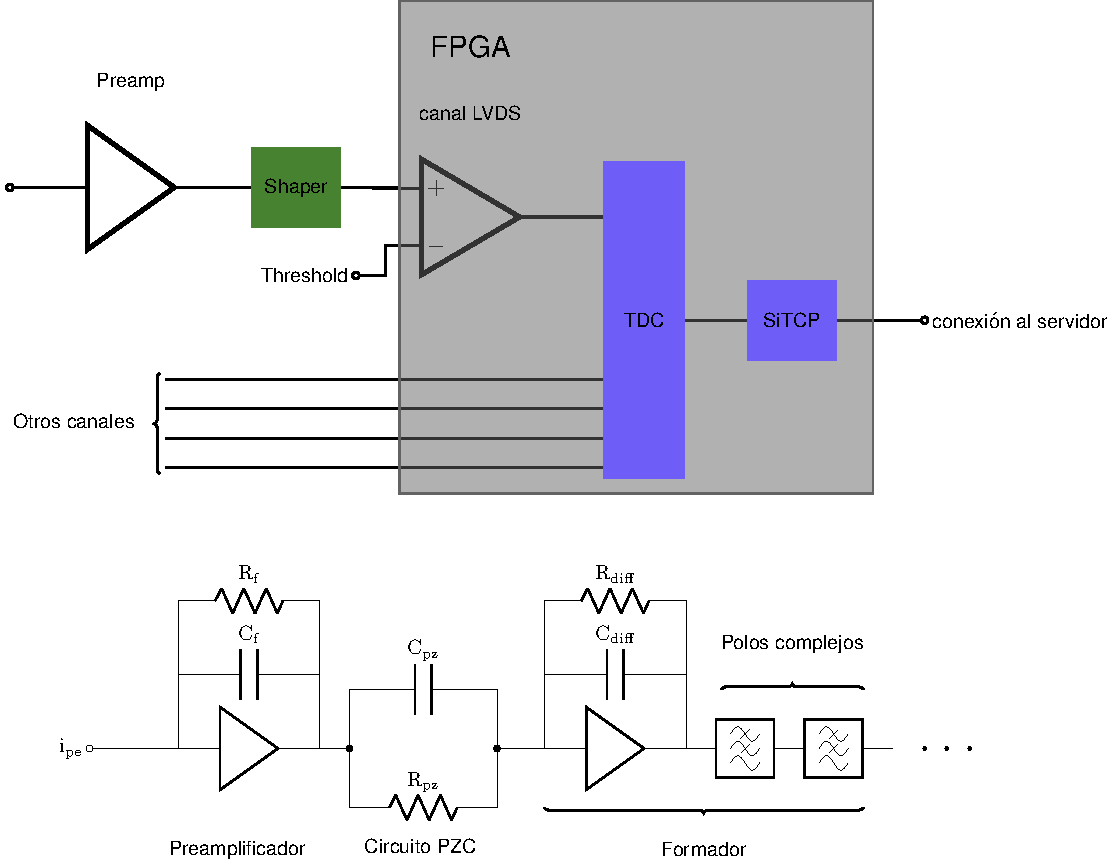
\includegraphics[width=\textwidth]{nfeb-prot.pdf}
        \caption{Diagrama esquemático de la nueva electrónica del SciCRT.}
        \label{fig:nfeb-prot}
\end{figure}

\section{Diseño de un \emph{Time digital converter} con sobremuestreo}

La arquitectura básica de un TDC está compuesta por un contador digital y un circuito detector de flancos (detección de inicio y fin de la señal a medir). A pesar de que este sistema puede tener un amplio rango dinámico de medición, la principal desventaja es la resolución temporal; ya que depende directamente de la frecuencia de reloj. Debido a esto resulta complejo en práctica alcanzar resoluciones temporales menores a \SI{10}{\nano\second} con esta arquitectura.

Un técnica empleada para superar esta limitación es el sobremuestreo \cite{spencer06,balla14}, cuyo principio de funcionamiento se ilustra en la figura \ref{fig:tdc-diagram}. Un TDC con sobremuestreo se compone de dos unidades: un contador grueso y un interpolador. El contador opera a una frecuencia $F_{0}=1/T_{0}$, con él se obtiene una medida \emph{entera} del número de ciclos de reloj que dura la señal a medir (en nuestro caso TOT). El interpolador se encarga de medir la parte fraccionaria del ciclo de reloj, utilizando para esto $N$ copias de la señal de reloj. Como se observa en la parte derecha de la figura \ref{fig:tdc-diagram}, las copias están retrasadas una respecto a la otra por un factor de $T_{0}/N$.  La lógica dentro del sistema interpolador se encarga de determinar cuál de las copias de la señal de reloj fue la primera en observar la transición de la señal a medir y fija un valor binario. El resultado de la medición del intervalo de tiempo es la suma la parte entera y la fraccionaria.

\begin{figure}
        \centering
        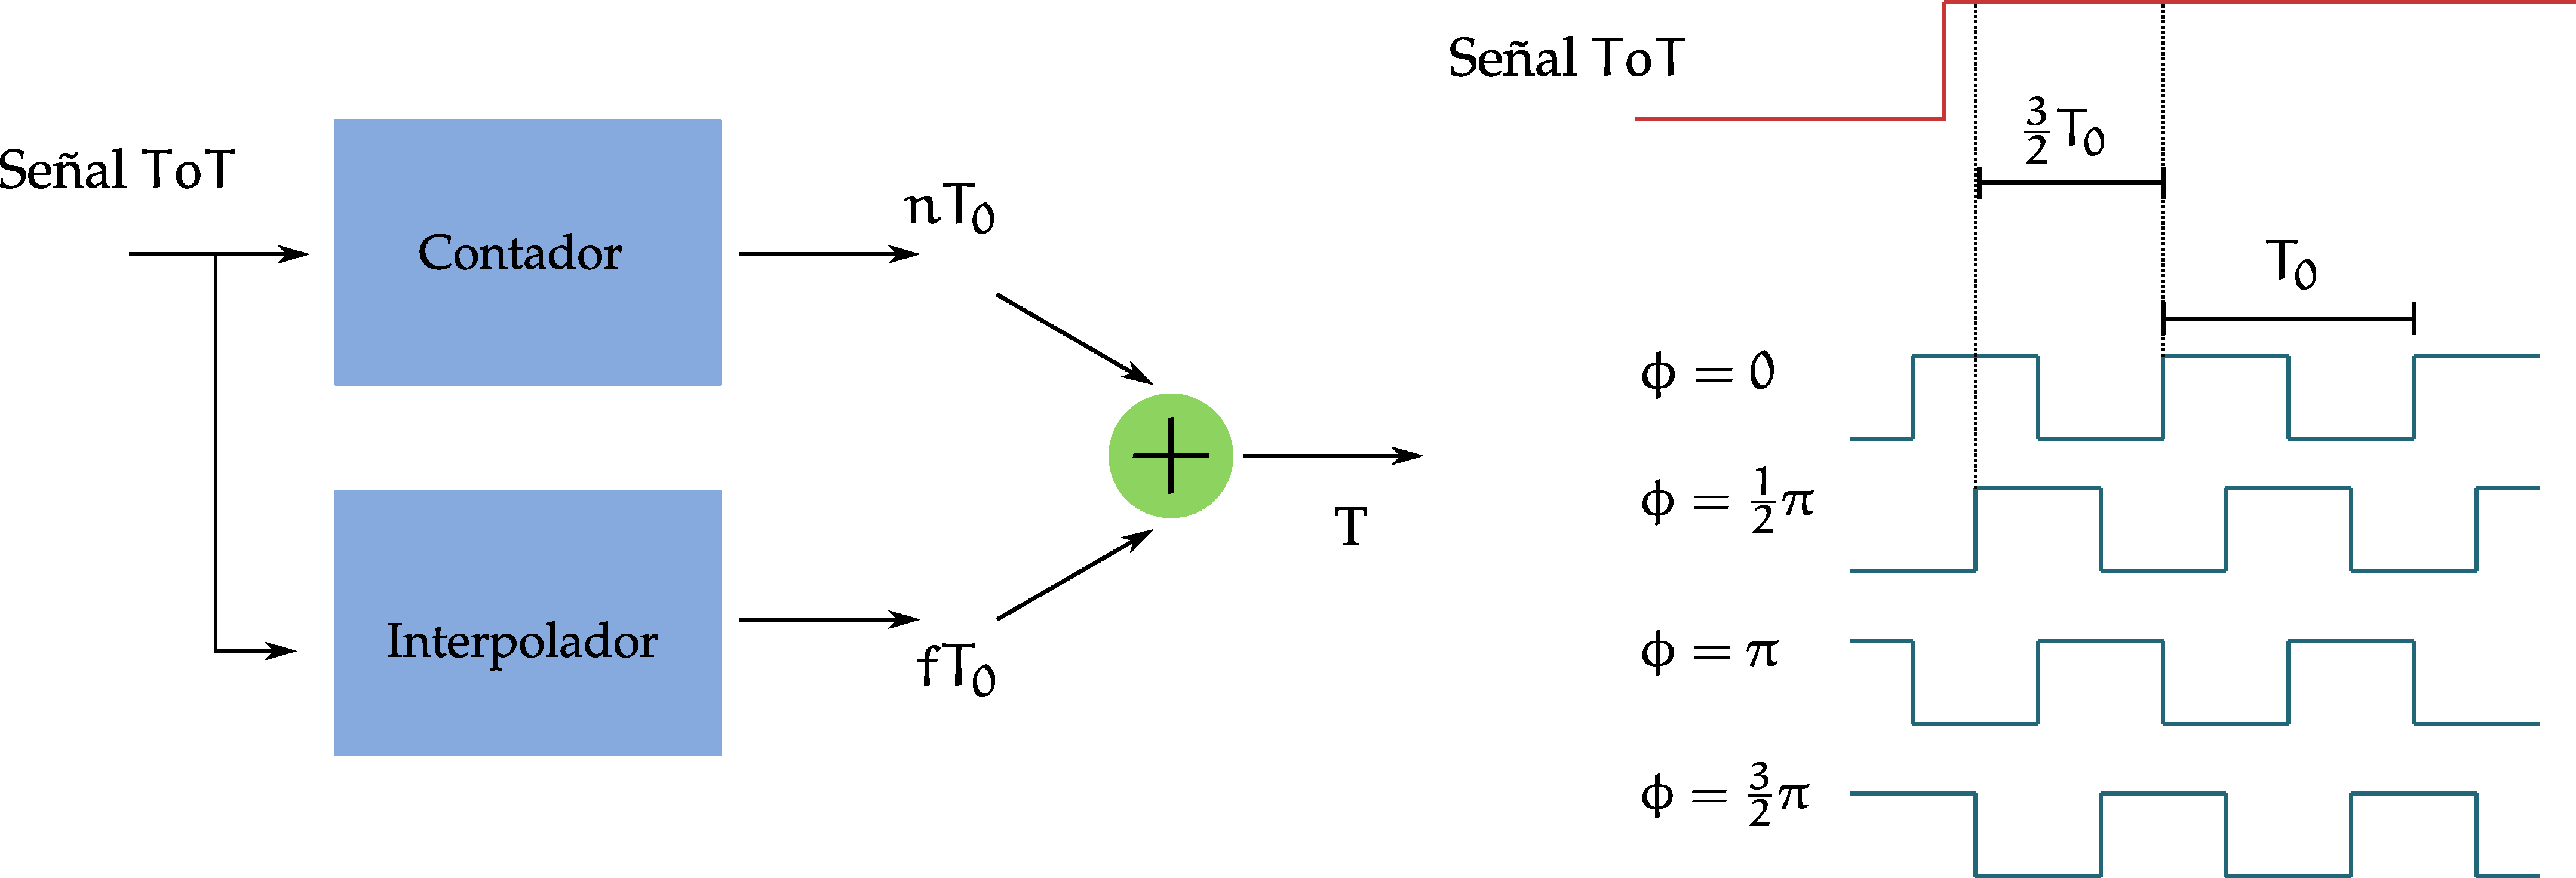
\includegraphics[width=\textwidth]{tdc-diagram.pdf}
        \caption{Arquitectura básica del sistema TDC por interpolación (panel izquierdo). Diagrama de tiempo y principio de operación del sistema TDC por interpolación.}
        \label{fig:tdc-diagram}
\end{figure}

Procedí a describir un módulo TDC en un FPGA usando un factor de sobremuestreo de \num{8}, con  pude obtener resoluciones temporales de \SI{0.5}{\nano\second} a \SI{2.5}{\nano\second}. En este modulo también incluí la transferencia de datos usando SiTCP. La precisión del convertidor fue medida usando una señal a la entrada de \SI{7.71}{\nano\second} de duración y una frecuencia de repetición de \SI{1}{\kilo\hertz}. En total obtuve una muestra de \num{1e5} eventos. La frecuencia de la señal a medir nos sirve para caracterizar el \emph{tiempo muerto} del sistema de adquisición y determinar si la velocidad de transmisión entre éste y la PC es suficiente para procesar la información obtenida del detector. Los resultados de la prueba se muestran en el histograma de la figura \ref{fig:tdc-lvds}.

\begin{figure}
        \centering
        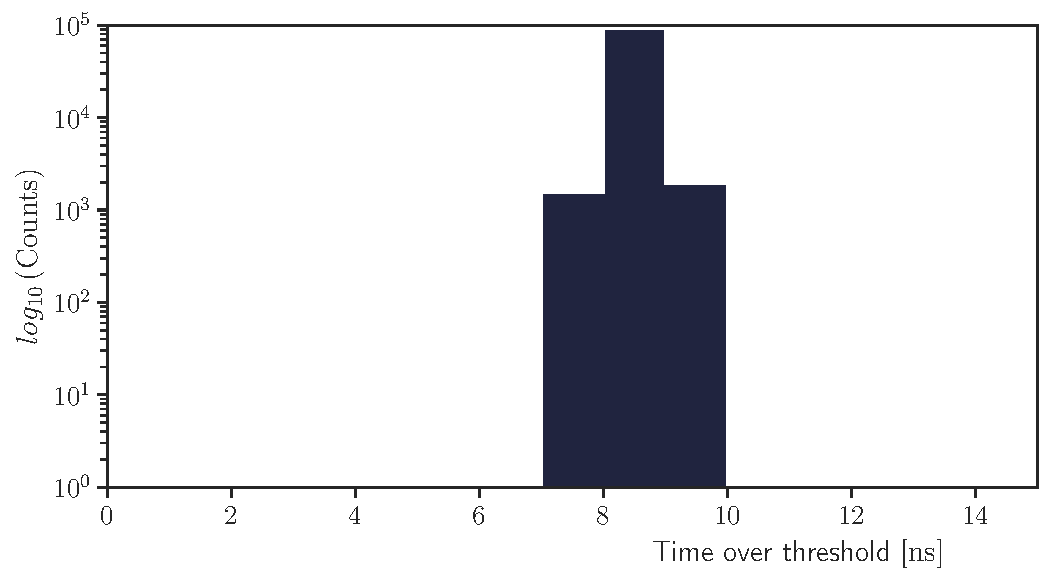
\includegraphics[width=\textwidth]{tot-lvds.pdf}
        \caption{Arquitectura básica del sistema TDC por interpolación (panel izquierdo). Diagrama de tiempo y principio de operación del sistema TDC por interpolación.}
        \label{fig:tdc-lvds}
\end{figure}

Al analizar los resultados de la figura, podemos concluir que son satisfactorios; ya que al utilizar un TDC con resolución de \SI{1}{\nano\second}, el \emph{bin} más cercano a la duración que deseamos medir es \SI{8}{\nano\second} y más del \SI{96}{\percent} de los eventos se encuentran en ese \emph{bin}. Solo el \SI{4}{\percent} de los eventos tienen una error producido debido a errores de sincronía del interpolador (los eventos entre \SI{7}{\nano\second} y \SI{9}{\nano\second}). Es importante mencionar que estos errores están directamente relacionados con el \emph{jitter} (fluctuaciones aleatorias en las fases) en la señal a medir y/o la señal de reloj.


\begin{figure}
  \centering
  \begin{subfigure}[b]{0.49\textwidth}
	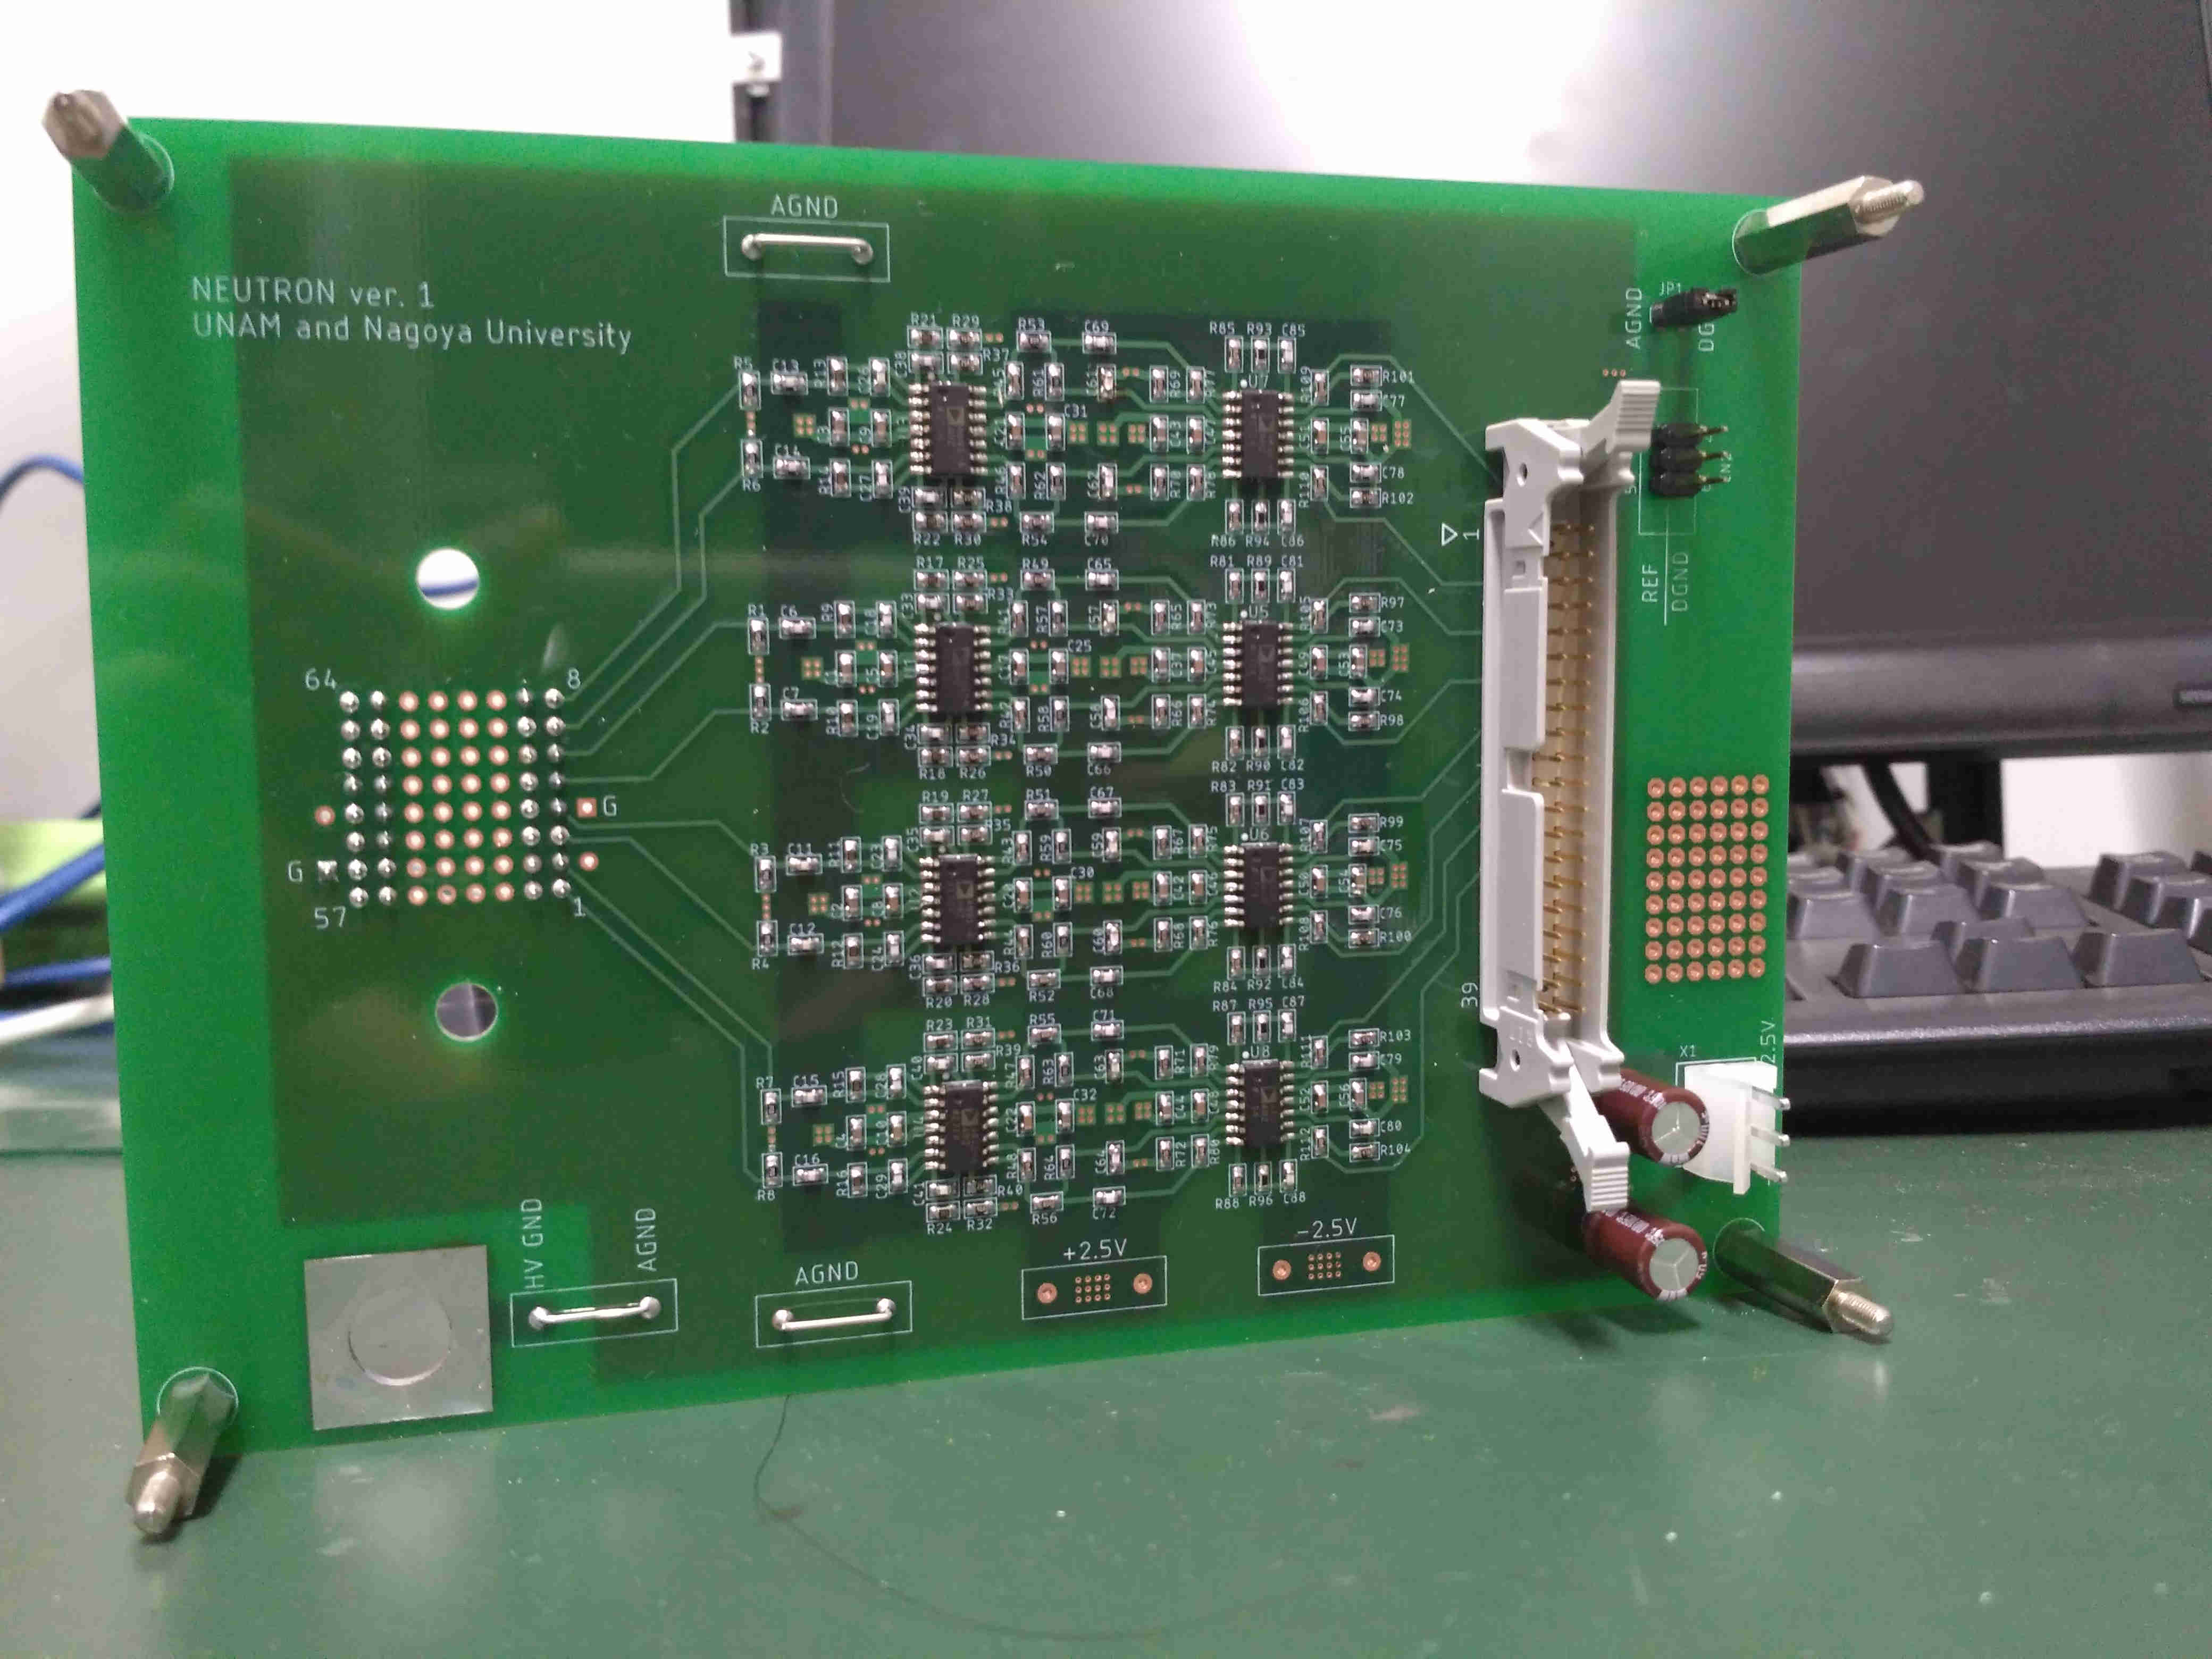
\includegraphics[width=\textwidth]{neutron_ver1.jpg}
	\caption{Tarjeta diseñada.}
	\label{fig:neutron-pcb}
  \end{subfigure}
  \begin{subfigure}[b]{0.49\textwidth}
	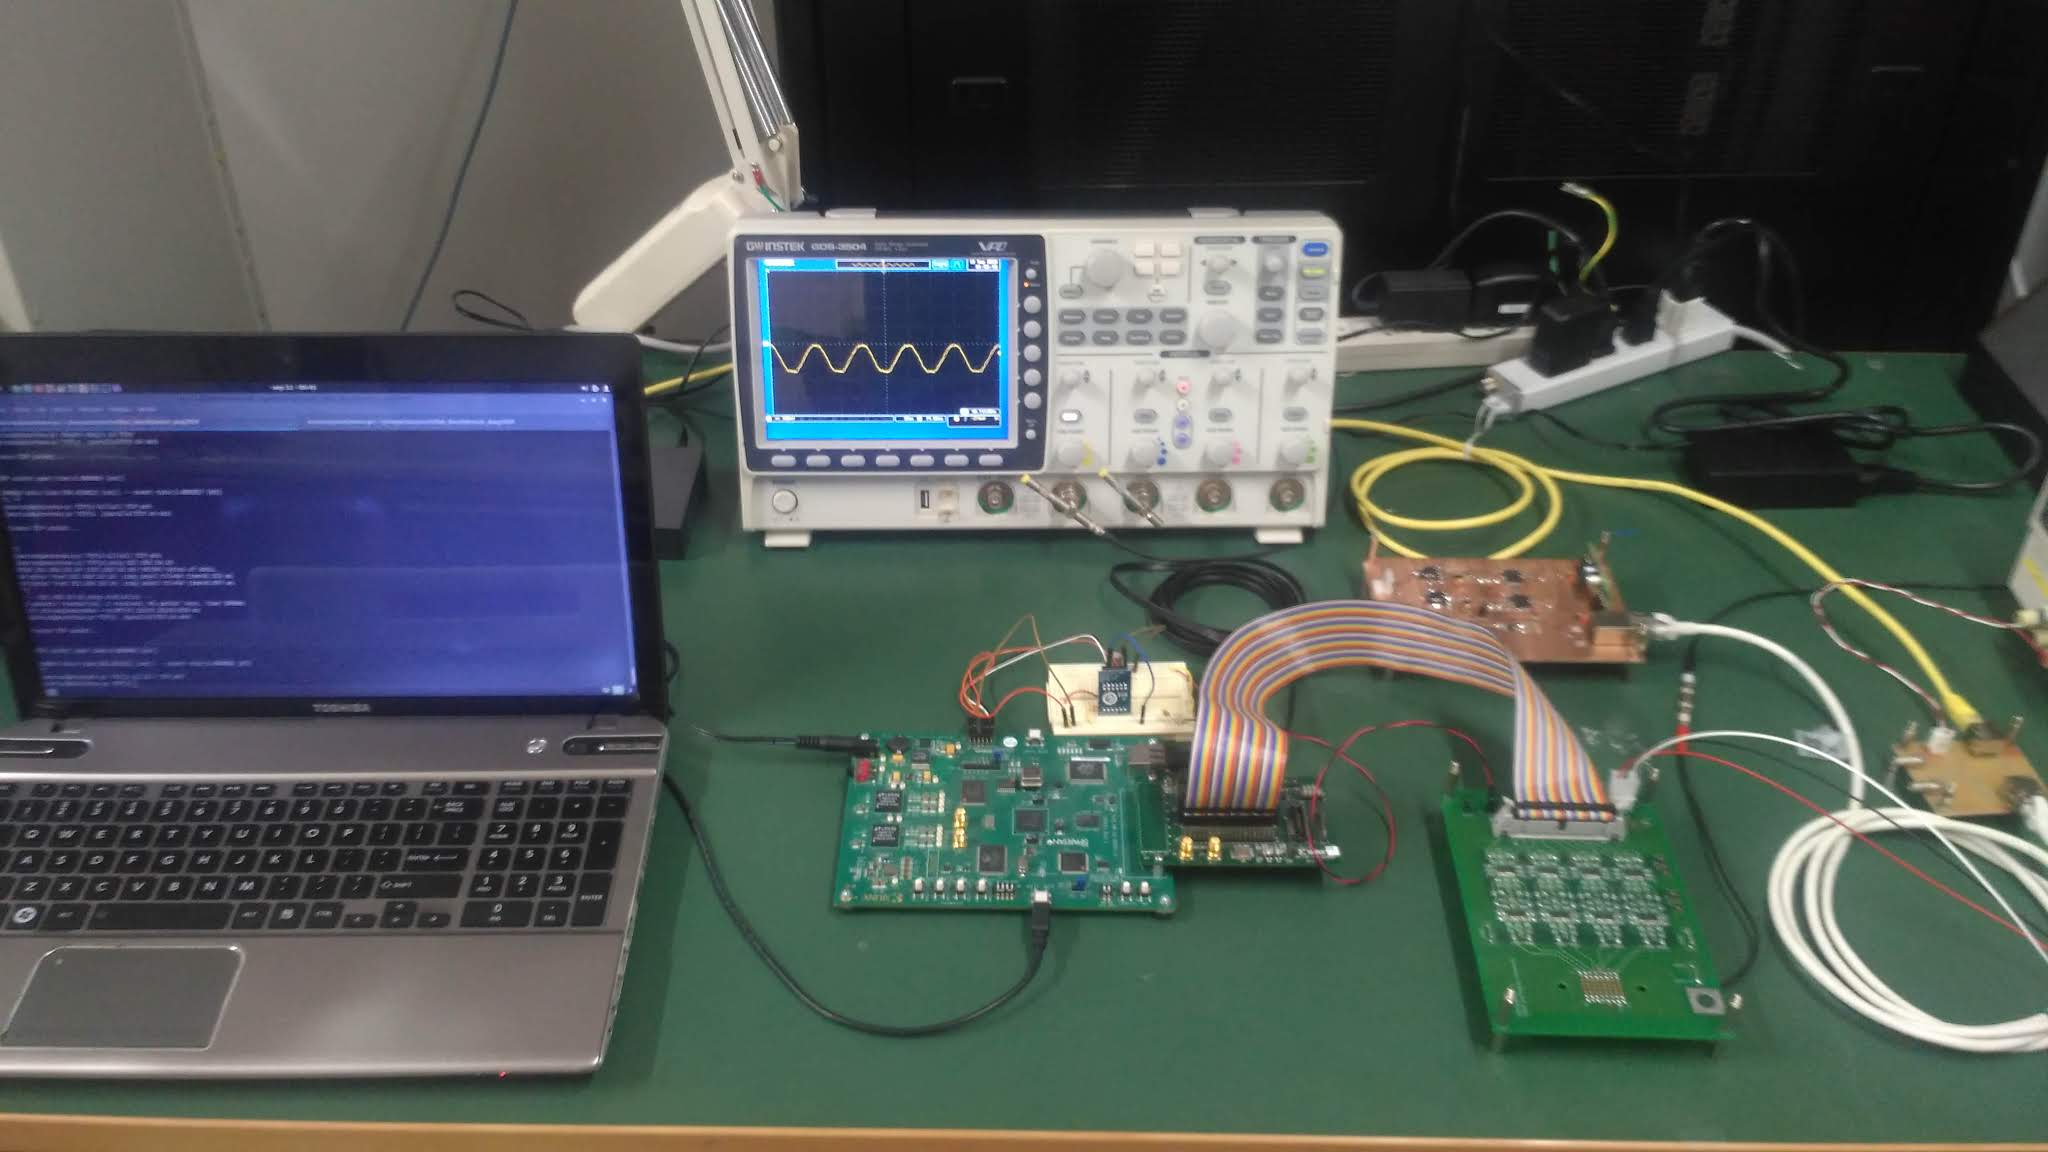
\includegraphics[width=\textwidth]{complete-system.jpg}
	\caption{Sistema en pruebas}
	\label{fig:complete-sys}
  \end{subfigure}
\end{figure}

\section{Diseño y optimización de la electrónica}



For the preamplifier unit we use an operational amplifier as charge sensitive amplifier with capacitor $C_{f}$ and resistor $R_{f}$ in the feedback loop. In principle, three parameters are needed for the specification of this system: values for $C_{f}$, $R_{f}$ and the minimum bandwidth of the amplifier. The $S/N$ ratio of the preamplifer is sensitive to both parameters, although in the case of the MAPMT the number of photo-electrons contained in the signal is of greater importance. Since MIPs in the far edge of the bar produce  \SI{10}{pe} in average (see next section for a description), we consider the effect of $C_{f}$, $R_{f}$ in the $S/N$ ratio negligible.

Las características del pulso después del procesamiento analógico (duración y amplitud) son afectadas directamente por el preamplificador, y debido a esto deben ser consideradas para la optimización del TDC. Un punto importante dentro de esto es la minimización del ruido de cuantización, lo cual puede alcanzarse utilizando de manera efectiva el rango dinámico del amplificador (buscando evitar la saturación) y el TDC. Para esto realizamos una simulación MC incluyendo la respuesta en frecuencia del preamplificador y el circuito formado (el cual se describe más adelante); variando el valor de $C_{f}$ en el rango de \num{10} a \SI{500}{\pico\farad}. De esta forma obtenemos la relación lineal entre el número de fotoelectrones en la pulso de entrada (\si{pe}) y la amplitud del pulso de salida. El valor de $R_{f}$ se selecciona en el rango de \num{1} a \SI{50}{\kilo\ohm} de forma que la constante de constante de integración sea aproximadamente \SI{600}{\ns}.

La figura \ref{fig:phe-cal} muestra el resultado de este análisis para $C_ {f}=20,40$ y \SI{100}{\pico\farad}, lo cual resulta en tres estructuras lineales distintivas. Los colores en la figura representan valores diferentes $R_{f}$ mientras $C_{f}$ permanece constante. Las líneas horizontales en la figura indican dos diferentes voltajes de saturación: \SI{5}{\volt} y \SI{2.5}{\volt}, correspondientes a dos diferentes tipos de amplificadores. A partir de esto podemos concluir que la pendiente de las curvas en la figura (la ganancia de conversión) es principalmente controlada por $C_{f}$, mientras que es relativamente insensible a cambios de$R_{f}$. Considerando que el rango dinámico de la señal de muones de \num{1} a \SI{250}{pe} (como se mostró en el capítulo \ref{chap:dos}), el valor óptimo para $C_{f}$ está entre \SI{20}{\pico\farad} y \SI{40}{\pico\farad}, en el caso de amplificadores con $V_{sat}=\SI{5}{\volt}$.

\begin{figure}
        \centering
        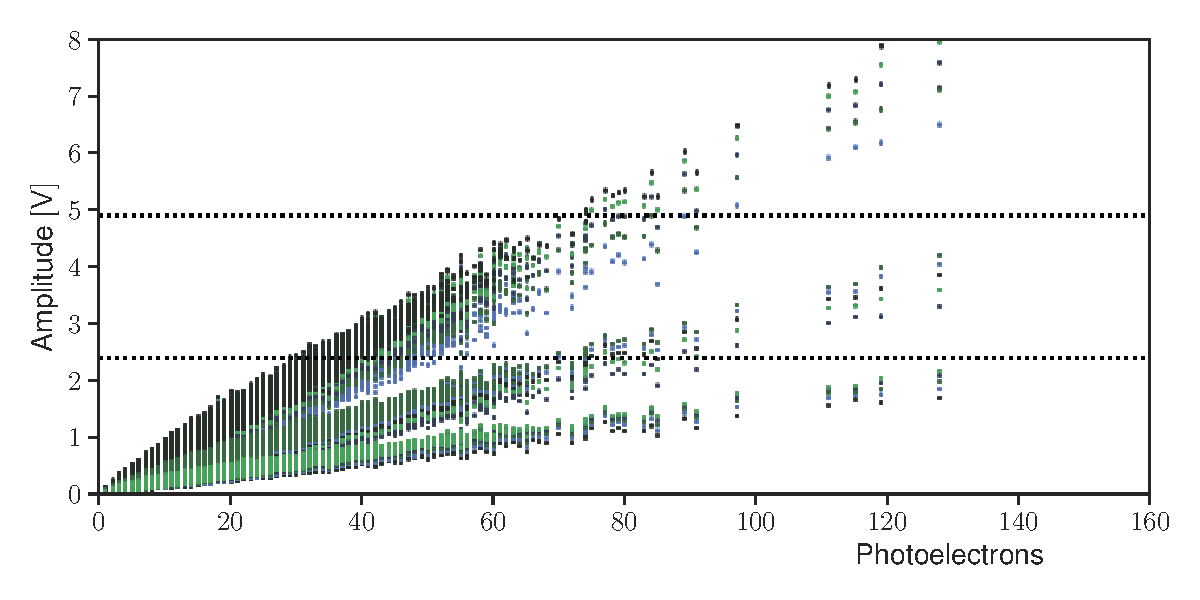
\includegraphics[width=\textwidth]{phe-cal.pdf}
        \caption{Respuesta del preamplificador en función de los elementos de realimentación. La ganancia de conversión. Los colores en la figura representan cambios en $R_{f}$ mientras $C_{f}$ se mantiene constante.}
        \label{fig:phe-cal}
\end{figure}

Lo siguiente es simular la conversión de la señal analógica a una señal $T_{OT}$. Primeramente,


 The conversion requires the definition of the shaping method as well as the resolution and range of the TDC. Along with the power consumption of the circuit, these last two parameters function as constrains to our optimization problem. The shaping method we use is the Gaussian filter because it is best suited for high speed performance \cite{ohkawa76}. Using the Gaussian shape as basis, the relation between the number of photo-electrons in the signal and the $T_{OT}$ can be written as:

\begin{equation}
\label{equ3.1}
T_{OT}^{2}=2\sigma^{2}\ln{k_{0} N_{phe}}-w_{th}
\end{equation}

where $N_{phe}$ is the number of photo-electrons, $k_{0}$ is the conversion gain of the preamplifier, $\sigma$ is the scaling parameter of the Gaussian and $w_{th}$ is an offset term, dependent of the threshold of the TOT and the $\sigma$. Using \ref{equ3.1}, taking into account that $k_{0}$ was determined in the previous step of our analysis, the characteristics of the muon signal may be effectively converted to digital time values changing the $\sigma$ of the shaper and/or the threshold of the system.

The full simulation of the electronics consider the preamplifier, shaping network and digital conversion by the TDC. The range and resolution of TDC are selected from the output of the simulation considering the cases were the full range of the muon signal occupies the most number of bins in the TDC. From this we conclude that a resolution of \SI{1}{\ns\per bin} and \SI{8}{bits \per sample} are enough for our application. Figure \ref{fig8} shows the results of the simulation with this resolution, for values of (from left to right) $\sigma=70,100$ and $\SI{125}{\ns}$. In each panel, the color scale represents different threshold values, starting with the highest at light blue and the lowest in light green. It is clear from the figure that the full dynamic range of the converter is achieved with $\sigma=\SI{125}{\ns}$.

To implement the shaping network we selected the method from  \cite{ohkawa76}. Under this framework, two parameters are required to specify the design: order $N$ of the filter and topology. We choose the Sallen-Key topology because it minimizes the gain-bandwidth product of the amplifier. The order of the filter improves the timing response of the shaping network and reduces the effect of pile-up, with the disadvantage of increasing power requirements. In the simulation we studied the case for shapers with $N=3$, $4$ and $5$ . Even without considering power constraints, the best performance in terms of dynamic range is achieved with $N=3$.

\begin{figure}
        \centering
        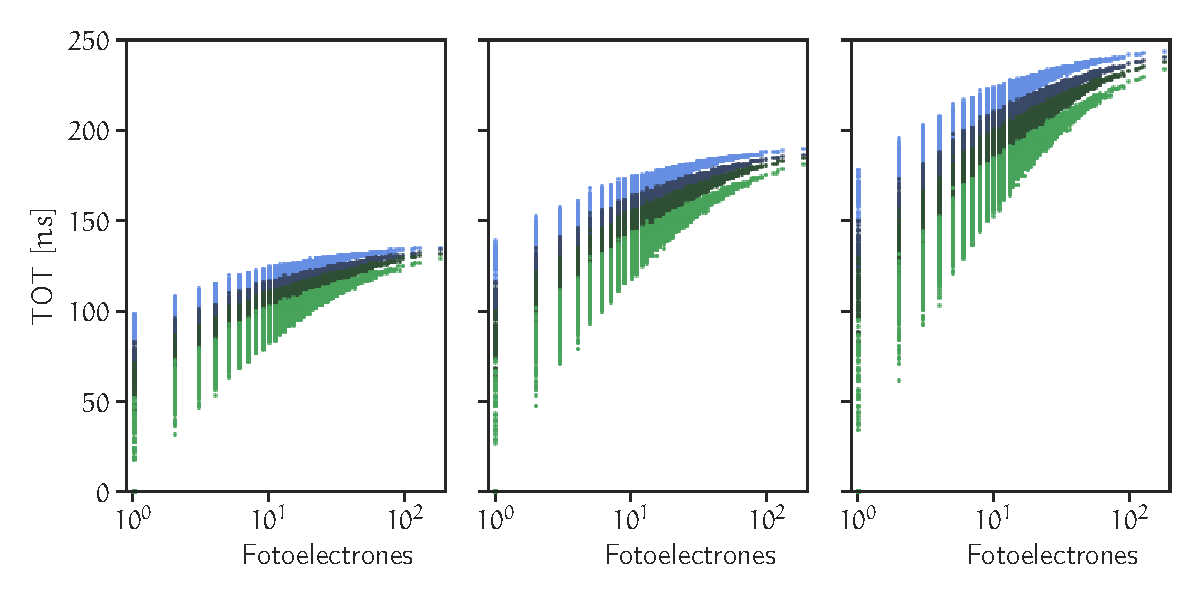
\includegraphics[width=\textwidth]{tot_d30par.pdf}
        \caption{Características del TOT para señales de muones simuladas usando formadores Gaussianos de diferente escala. El panel de la izquierda es con $\sigma=70$, el panel del centro corresponde a $\sigma=100$ y el panel de la derecha es $\sigma=125$. Los colores representan cambios en el umbral, desde \SI{10}{\milli\volt} (azul claro) a \SI{50}{\milli\volt} (verde claro).}
        \label{fig:tot-sigma}
\end{figure}


\begin{figure}
        \centering
        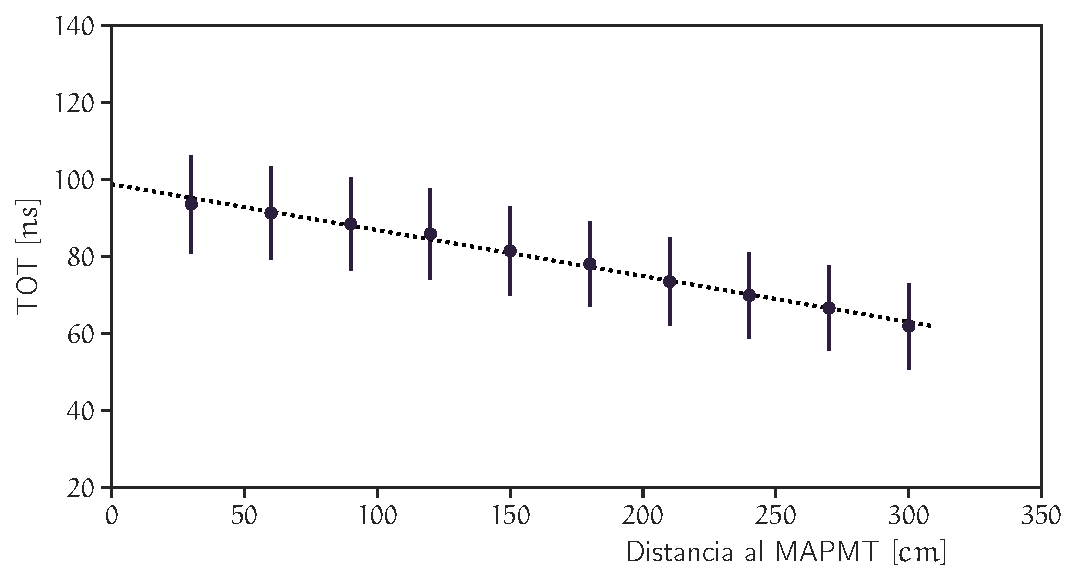
\includegraphics[width=\textwidth]{tot_distance.pdf}
        \caption{Valores promedio de TOT a diferentes distancias del MAPMT, incluyendo barras de error de $\pm\sigma$. La línea punteada representa el resultado del ajuste lineal.}
        \label{fig:tot-distance}
\end{figure}

\begin{figure}
        \centering
        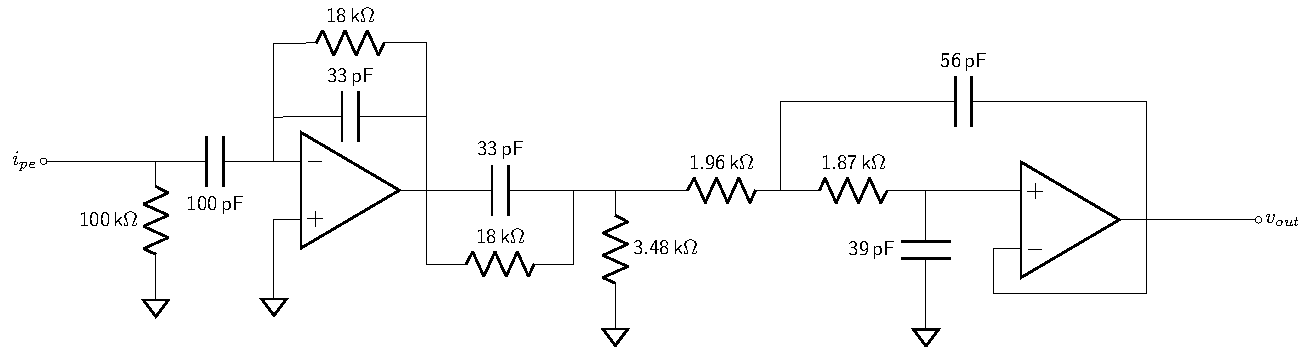
\includegraphics[width=\textwidth]{preamp-shaper-final.pdf}
        \caption{Diagrama esquemático del circuito preamplificador/formador. Para el análisis mediante la simulación MC consideramos dos modelos de amplificadores: ADA4891 y ADA4807.}
        \label{fig:preamp-shaper}
\end{figure}

\begin{figure}
        \centering
        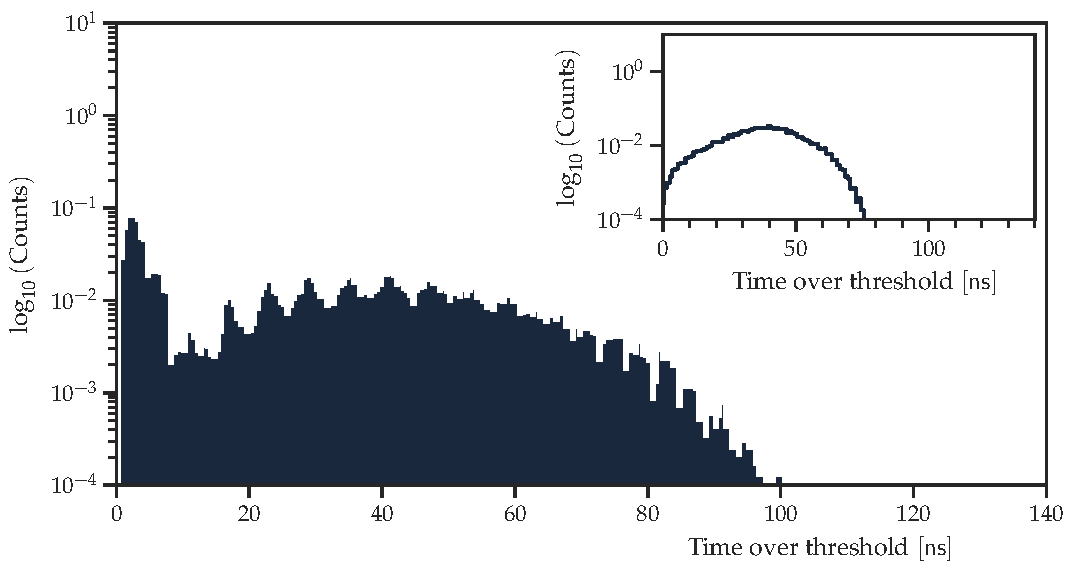
\includegraphics[width=\textwidth]{tdc_sim-exp.pdf}
        \caption{Distribución experimental de TOT (lienzo grande) y simulación (canvas pequeño) para una carga equivalente de \SI{10}{pe} utilizando un TDC de \SI{8}{\bit} con \SI{1}{\ns} resolution.}
        \label{fig:tdc-simexp}
\end{figure}
